\section{Graphviz}
\fib{}
\subsection{Allgemeines}

\noindent
Graphviz ist eine Open-Source Software mit der man Graphen darstellen kann.
Entwickelt wurde es von AT\&T und den Bell Labs, die es zum Ersten mal in den 1990er veröffentlichten. Die aktuellste Version von Graphviz ist die Verion 2.41 und wurde am 25.Dezember 2016 veröffentlicht. Graphviz ist dazu da aus strukturierten Daten gerichtete oder ungerichtete Graphen zu generieren. 
\footcite{graphviz_nodate}

\noindent
Außerdem wird Graphviz in Programmen verwendet wie in z.B.:
\begin{itemize}
	\item AsciiDoc
	\item PlantUML
	\item Trac
	\item Sphinx
\end{itemize}
\noindent
Wobei die letzten beiden Programme im laufe des Projekts verwendet wurden.

\noindent
In drei von vier Ausgabeformaten dieses Projekts kommt Graphviz zum Einsatz. In einem Ausgabeformat, um damit selbst die Modelle zu generieren und in den anderen zwei Ausgabeformaten, um an die Koordinaten zu kommen an denen die Elemente positioniert werden müssen.

\subsubsection{Ablauf des Programms}

\noindent
\lstset{language=Python}
\lstset{frame=lines}
\lstset{caption={Programmcode, um einen Graphen anzulegen}}
\lstset{label={create_graph}}
\lstset{basicstyle=\footnotesize}
\begin{lstlisting}

name = "erd"
set = False
for child in _root:
if child.tag == "title":
name = child.get("name")
set = True
if set:
break
_erd = Graph(name, filename=name, engine="sfdp")
self.create_erd(args, _erd, _root)

\end{lstlisting}
\noindent
Im Listing \ref{create_graph} sieht man wie ein leerer Graph, der nur einen Namen und eine Engine besitzt, erstellt wird. 
Die Variable ``set,, verhindert das mehrfache setzen vom Namen des Graphen. 

\noindent
Für die Darstellung eines Entity-Relationship Diagramms werden folgende Formen benötit:
\begin{itemize}
	\item Raute (einfach umrandet oder doppelt umrandet)
	\item Rechteck (einfach umrandet oder doppelt umrandet)
	\item Ellipse (einfach umrandet oder strichliert umrandet)
	\item Dreieck (schwarz ausgemahlt oder leer)
\end{itemize}


\begin{figure}[H]
	\begin{center}
		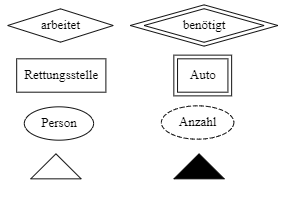
\includegraphics[width=16cm,height=10cm]{images/graphviz_formen.png}
		\caption{Formen in Graphviz}
		\label{dot}
	\end{center}
\end{figure}
\fib{}
\noindent
Diese Elemente werden dann mit Linien verbunden. Diese können im speziellen Fall einer totalen Vererbung auch als doppelte Linie vorkommen.
\lstset{language=Python}
\lstset{frame=lines}
\lstset{caption={Programmcode, um Entities zu erstellen}}
\lstset{label={create_ent}}
\lstset{basicstyle=\footnotesize}
\begin{lstlisting}

def create_ent(self, erd, name, weak):
if not weak:
erd.attr("node", shape="box", peripheries="1")
erd.node(name)
else:
erd.attr("node", shape="box", peripheries="2")
erd.node(name)

\end{lstlisting}
\noindent
Um einen Entity-Typen zu zeichnen muss vorher der Name des Entity-Typen und ob er abhängig oder nicht abhängig ist bekannt sein. Außerdem muss der Graph in dem das Element sich befindet mitgegeben werden. Wie man im Listing \ref{create_ent} sieht wird durch eine if-Verzweigung darüber entschieden ob ein Rechteck mit doppeltem Rand oder einfachem Rand erstellt wird. Dementsprechend werden die Eigenschaften von ``erd.attr,, mit dem Namen node angepasst.
\newpage
\fib{}
\noindent
\lstset{language=Python}
\lstset{frame=lines}
\lstset{caption={Programmcode, um Attribute zu erstellen}}
\lstset{label={create_attr}}
\lstset{basicstyle=\footnotesize}
\begin{lstlisting}

def create_attr(self, erd, name, prime, label):
if prime:
erd.attr("node", shape="ellipse", style="dashed", label=label)
erd.node(name)
else:
erd.attr("node", shape="ellipse", label=label)
erd.node(name)

\end{lstlisting}
\noindent
Bei dem Erstellen der Attribute muss zusätzlich zu Name und in welchem Graphen es sich befindet, auch bekannt sein ob es sich um einen Primär-Schlüssel handelt und zu welchem Entity-Typen das Attribut gehört. Der Parameter ``label,, ist der Name des Attributs und der Parameter ``name,, ist der Name von dem dazugehörigen Entity-Typen. Durch den Parameter ``prime,, wird in der if-Verzweigung, die man im Listing \ref{create_attr} sieht, ob es sich um einen Primär-Schlüssel handelt. Falls dem so ist wird die Ellipse mit strichliertem Rand erstellt.

\noindent
\lstset{language=Python}
\lstset{frame=lines}
\lstset{caption={Programmcode, um Beziehung zu erstellen}}
\lstset{label={create_rel}}
\lstset{basicstyle=\footnotesize}
\begin{lstlisting}

def create_rel(self, erd, name, weak, sup, disjoint):
if weak:
erd.attr("node", shape="diamond", peripheries="2")
erd.node(name)
elif sup:
if disjoint:
erd.attr("node", shape="triangle", color="black")
erd.node(name=name, style="filled")
else:
erd.attr("node", shape="triangle", color="white")
erd.node(name=name, style="filled")
else:
erd.attr("node", shape="diamond", peripheries="1")
erd.node(name)

\end{lstlisting}
\noindent
Für die Erstellung von den Beziehungen zwischen zwei Entity-Typen muss man angeben ob es sich um eine abhängige Beziehung handelt oder nicht, außerdem muss noch angegeben werden ob eine Vererbung vorliegt und wenn ja ob sie disjunkt oder nicht disjunkt ist. Wie man im Listing \ref{create_rel} sieht wird zunächst unterschieden, ob die Beziehung einer Vererbung angehört, einem abhängigen Entity-Typen angehört oder ob sie eine gewöhnliche Beziehung zwischen zwei Entity-Typen ist. Je nachdem wird dann entweder eine Raute oder ein Dreieck erstellt. Außerdem wird darüber entschieden ob das Dreieck schwarz gefüllt ist oder weiß ist. Der Beziehung ist zu diesem Zeitpunkt nicht bekannt mit welchen Linien sie mit welchen Entity-Typen verbunden wird.
\newpage
\fib{}
\noindent
\lstset{language=Python}
\lstset{frame=lines}
\lstset{caption={Programmcode, um Formen zu verbinden}}
\lstset{label={create_line}}
\lstset{basicstyle=\footnotesize}
\begin{lstlisting}

def create_edgeTotal(self, erd, ent1, ent2):
erd.edge(ent1, ent2, peripheries="2")

def create_edgeRel(self, erd, ent1, ent2, mini, maxi):
s = "(" + mini + ", " + maxi + ")"
erd.edge(ent1, ent2, label=s, peripheries="1")

def create_edge(self, erd, ent1, ent2):
erd.edge(ent1, ent2, peripheries="1")

\end{lstlisting}
\noindent
\begin{itemize}
	\item Um gewöhnliche Entity-Typen mit einem normalen Beziehungs-Typen zu verbinden wird die Funktion ``create edgeRel,, verwendet. Dabei werden die beiden Formen im Graphen mitgegeben, der Graph selbst und min und max werte des Beziehungs-Typen.
	\item Im Falle einer Vererbungen mit einer totalen Beziehung wird die Funktion ``create edgeTotal,, verwendet.  Dabei werden nur die beiden Formen im Graphen mitgegeben und der Graph selbst.
	\item Für jeden anderen Fall wird die Funktion ``create edge,, verwendet aber wird diese Funktion am häufigsten beim verbinden der Attribute  mit dem dazugehörigen Entity-Typen.
\end{itemize}

\noindent
\lstset{language=Python}
\lstset{frame=lines}
\lstset{caption={Programmcode, um Formen zu verbinden}}
\lstset{label={create_line}}
\lstset{basicstyle=\footnotesize}
\begin{lstlisting}

erd.render(format="pdf")
cwd = os.getcwd()
print("Your ERD is sucessfully created in:" + cwd)

\end{lstlisting}

\noindent
Nachdem der Graph und die Formen erstellt wurden und die Formen miteinander verbunden wurden. Wird das Dateiformat angegeben in welchem der Graph ausgegeben werden soll. Außerdem wird das Verzeichnis in dem die Datei gespeichert wird auf der Konsole ausgegeben.


\newpage
\subsection{Dateiformate}
\fib{}
\noindent
Graphviz bietet standardmäßig eine Vielzahl an verschiedenen Datei- oder Output-Formaten an.
Insgesamt sind es 55 verschiedene Formate und allein davon sind sechs Formate Variationen des ``dot,, Formats. Für dieses Projekt wurden hauptsächlich das PDF-Format genutzt. Das PIC-Code-Tool verwendete jedoch das ``pic-Format,, um die Koordinaten des Graphen mittels Graphviz zu ermitteln und an das Tool weiterzuleiten.
\footcite{noauthor_output_nodate}
Zu den gängigsten Datenformaten zählen:
\begin{itemize}
	\item dot
	\item bmp
	\item json
	\item pdf
	\item svg
	\item png
\end{itemize}

\subsubsection{dot-Format}
Die Ausgabe dieses Formats und der Formate gv, xdot, xdot1.2 und xdot1.4, erfolgt in dot-language. 
Darin stehen dann die Attribute für:
\begin{itemize}
	\item Begrenzungsrahmen
	\item Position
	\item Breite
	\item Höhe
	\item Labelpunkt
\end{itemize}
\noindent
Außerdem gibt es dann noch die Attribute ``rects,, und/oder ``vertices,, und noch weitere je nachdem welche Formen im Graphen angezeigt werden.

\subsubsubsection{xdot}
\noindent
``xdot,, steht für ``extended dot,, und ist einfach eine erweiterte Version von dot, die genauere Daten über den Graph zurück liefert als dot.
Kommentare für die Lesbarkeit und für das Verständnis kann man schreiben. Weiteres gibt es auch das Attribute ``xdotversion,, um Änderungen am Graphen zu erlauben. 

\subsubsubsection{xdot1.4}
\noindent
Mit``xdot1.4,, können Farbstrings lineare und radiale Farbverläufe codieren.
\begin{itemize}
	\item Lineare-Form:  '[' x0 y0 x1 y1 n [color-stop]+ ']'
	\item Radiale-Form:  '(' x0 y0 r0 x1 y1 r1 n [color-stop]+ ')' 
\end{itemize}
\noindent
Die Zahl n gibt an wie viele Color-stop es gibt. 
Wenn eine Form keine Farbe besitzt kann zu ihr auch keine Verbindung erstellt werden, auch wenn sie theoretisch existiert.


\newpage
\fib{}
\subsubsection{json}
\noindent
Dateiformate die JSON als ausgabe haben:
\begin{itemize}
	\item json
	\item json0
	\item dot json
	\item xdot json
\end{itemize}
\noindent
Bei Verwendung des Formats ``json,, bekommt man das selbe Ergebniss wie bei dem Format ``-Txdot,, nur als JSON anstelle einer Datei in DOT language. Genauso verhält es sich auch bei ``json0,, und ``-Tdot,,. Die Formate ``dot json,, und ``xdot json,, sind ``json0,, und ``json,, ähnlich. Jedoch verwenden diese zwei Formate nur die Input Daten und somit ist bei ihnen kein Layout durch einen bestimmten Algorithmus vorgegeben, dadurch enthalten diese Formate nur die Information über die Elemente selber.
Die daraus entstehende JSON-Datei kann wie folgt aufgebaut sein wie im Listing \ref{json}.

\noindent
\lstset{language=python}
\lstset{frame=lines}
\lstset{caption={Beispiel für eine JSON Datei von Graphviz}}
\lstset{label={json}}
\lstset{basicstyle=\footnotesize}
\begin{lstlisting}

{
"nodes": [
{
"id": "n0",
"label": "A node",
"x": 0,
"y": 0,
"size": 3
},
{
"id": "n1",
"label": "Another node",
"x": 3,
"y": 1,
"size": 2
},
],
"edges": [
{
"id": "e0",
"source": "n0",
"target": "n1"
},
{
"id": "e2",
"source": "n1",
"target": "n0"
}
]
}

\end{lstlisting}

\subsubsection{pdf}
\noindent
Das Format ``pdf,, erstellt ein PDF-Dokument.
Falls man Anker benutzen möchte sollte man als alternative das Format ``ps2,, benutzen, da das mit diesem möglich ist und dem Format ``pdf,, ähnelt.

\subsubsection{plain-ext}
\fib{}
Die Formate ``plain,, und ``plan-ext,, geben ein Text-Dokument aus dieses besteht aus vier verschiedenen Arten von Zeilen:
\begin{itemize}
	\item graph
	\item node
	\item edge
	\item stop
\end{itemize}
\noindent
Die ``stop,, Zeile markiert das Ende eines Graphen. Die Ausgabe besteht aus einer Zeile für den Graphen, mehreren Zeilen für Elemente, pro Element keine bis mehrere Zeilen für die Verbindungen und am Ende befindet sich ein Stop.

\subsubsubsection{graph}
\noindent
Die ``graph,, Zeile gibt die Breite sowie die Höhe des Graphen mit den Attributen ``height,, und ``width,, an. Wenn der Graph skaliert werden muss gibt es ein Attribute ``scale,,. Dieses Attribute gibt an in welchem Verhältnis der Graph skaliert werden muss. Außerdem sind alle Werte nicht skaliert was bedeutet, wenn der Wert des Attributes ``scale,, nicht 1.0 ist muss jede Zahl damit multipliziert werden. Standardmäßig ist der Koordinatenursprung in der linken unteren Ecke.

\subsubsubsection{node}
\noindent
Die ``node,, Zeilen besitzt die Attribute ``name,, welches dem Element seinen Namen verleiht, ein ``x,, und ein ``y,, Attribute welche die Position des Elements festlegen. Außerdem wird die Breite sowie die Höhe des Element, wie bei dem ``graph,, Statement mit den Attributen ``height,, und ``width,, angegeben. Außerdem verfügt es auch noch über die Attribute ``label,,, ``style,,, ``shape,,, ``color,, und ``fillcolor,,. Wenn das ``style,, Attribute leer ist, ist der Rahmen des Elements Standardmäßig solide.

\subsubsubsection{edge}
\noindent
Die zwei wichtigsten Attribute der ``edge,, Zeile sind ``tail,, und ``head,,, diese geben die zwei Namen der zu verbindenden Elemente an.

\subsubsection{png}
\noindent
Das ``png,, Format ist eines der unpraktischsten dafür einfachsten Formate da es lediglich ein Bild zurück liefert.
Jedoch kann man bei diesem Format einstellen ob das Bild mit Antialiasing generiert werden soll oder ohne. Außerdem kann man auch noch angeben ob es mit ``Indexed color,, oder mit ``True color,, generiert werden soll. 

\newpage
\subsection{Engines}
\fib{}
\noindent
Die sogenannten Engines in Graphviz geben an mit welchem Verfahren die Koordinaten der Elemente berechnet werden. Das kann von großem Vorteil sein wenn man bestimmte Ergebnisse erzielen will.
\footcite{noauthor_documentation_nodate}

\subsubsection{dot}

\noindent
dot ist in erster Linie dafür gedacht Strukturen hierarchisch abzubilden. Das bedeutet das dabei alle Kanten in etwa die selbe Richtung verlaufen, meistens von oben nach unten oder von links nach rechts. Durch diese Anordnung der Elemente kommt es selten zu Kanten Überschneidungen da sie auch in der Regel eher kurz gehalten werden.
Daher wird man eher dot verwenden wenn man weiß, dass die Kanten eine Richtung besitzen.

\begin{figure}[H]
	\begin{center}
		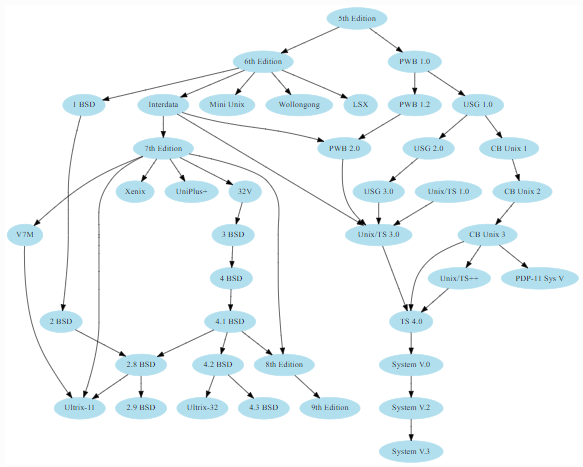
\includegraphics[width=16cm, height=10cm]{images/dot.png}
		\caption{Typischer dot Graph}
		\label{dot}
	\end{center}
\end{figure}
\footcite{noauthor_graphics_nodate}
\newpage
\noindent
\subsubsection{neato}
\fib{}
\noindent
neato benutzt das sogenannte ``spring model,, Layout. Neato benutzt den Kamada-Kawai-Algorithmus und ist eher dafür gedacht kleinere Graphen(um die 100 Knoten) darzustellen. Man benutzt Neato dann wenn man nichts außer der Größe des Graphen kennt. Neato führt einen Vorgang durch, beim generieren des Graphen, der äquivalent zu Multi-Dimensionaler Skalierung ist.
\footcite{north_drawing_2004}
\begin{figure}[H]
	\begin{center}
		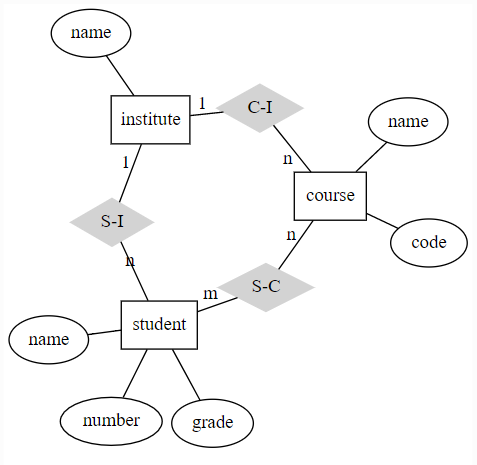
\includegraphics[width=14cm, height=8cm]{images/neato.png}
		\caption{Typischer neato Graph}
		\label{neato}
	\end{center}
\end{figure}

\noindent
\subsubsection{fdp}

\noindent
fdp benutzt genau wie neato auch das ''spring model,, Layout. Jedoch wendet es ein anderes Verfahren an.

\subsubsection{sfdp}

\noindent
sfdp benutzt genau wie fdp und neato auch das ''spring model,, Layout. Außerdem ist sdfp eine multiscale Variante von fdp mit der man sehr große Graphen darstellen kann.
\footcite{noauthor_performance_nodate}
\begin{figure}[H]
	\begin{center}
		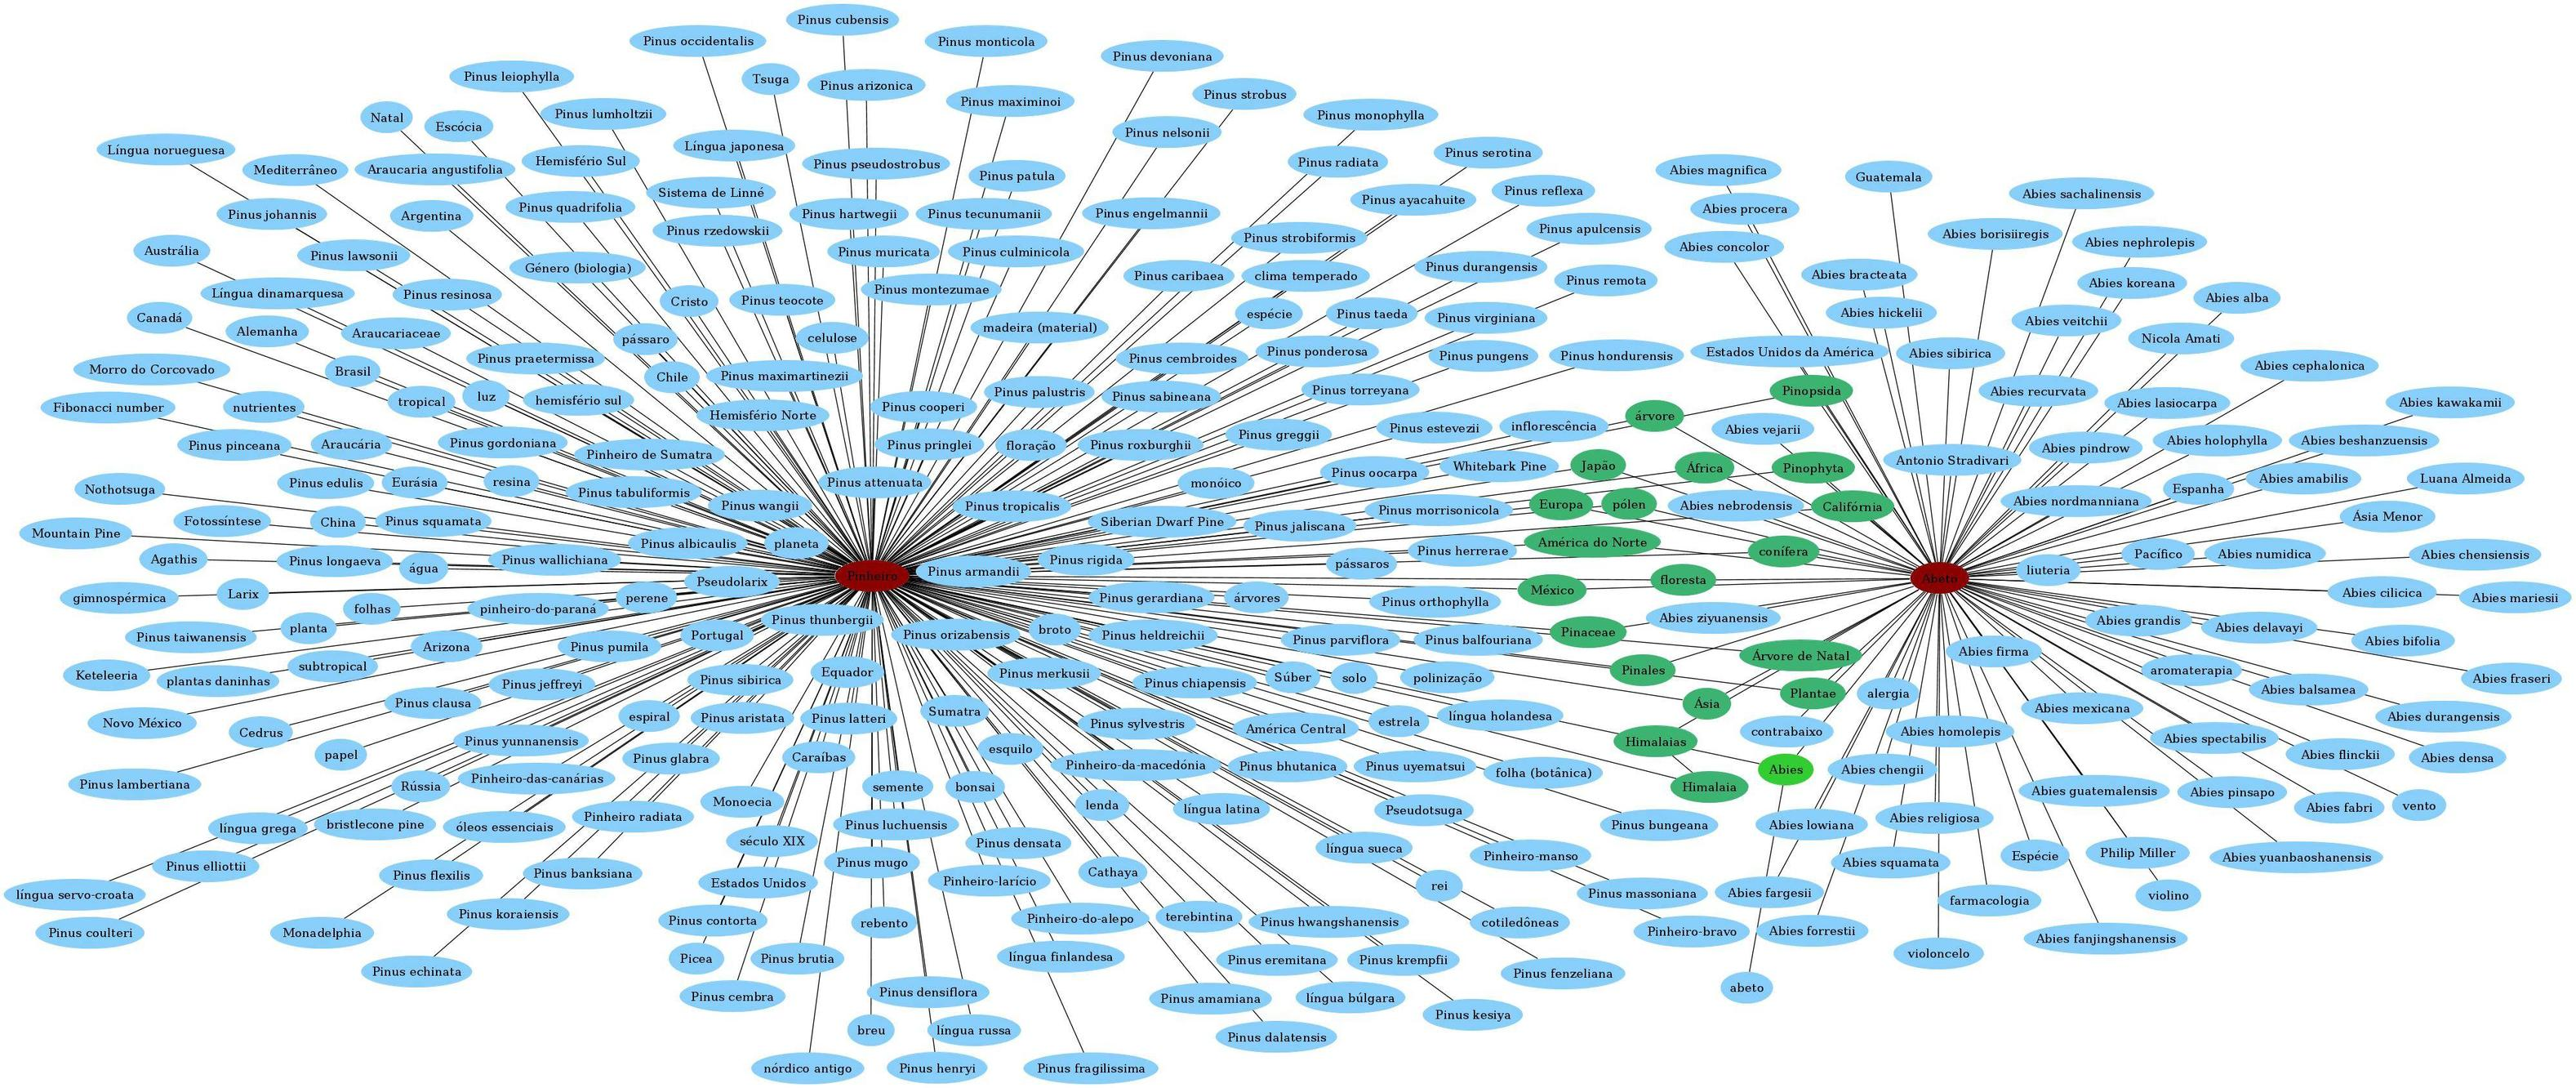
\includegraphics[width=14cm, height=8cm]{images/sfdp.jpg}
		\caption{Typischer sfdp Graph}
		\label{sfdp}
	\end{center}
\end{figure}

\noindent
\subsubsection{circo}
\fib{}
\noindent
circo erstellt ein circuläres Layout nach Six und Tollis 99, Kauffman und Wiese 02. Dieses Verhalten verlieh ihm auch seinen Namen. Diese Art von Graphen Generierung ist dazu geeignet Zyklische Strukturen, wie man sie meist bei Telekomunikations-Netzwerken vorfindet, darzustellen.

\begin{figure}[H]
	\begin{center}
		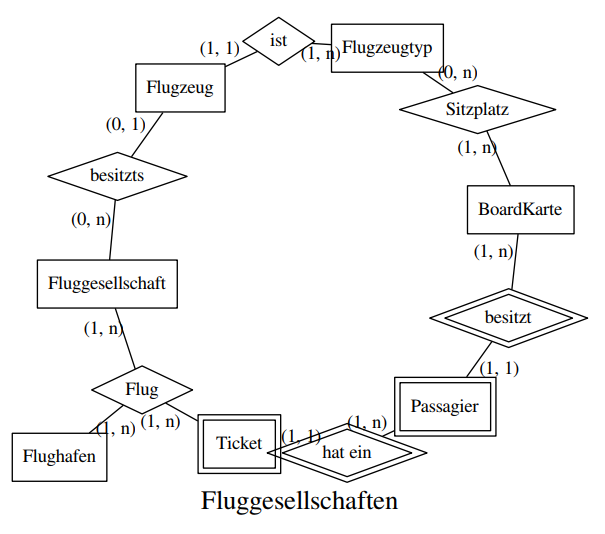
\includegraphics[width=14cm, height=8cm]{images/circo.png}
		\caption{Typischer circo Graph}
		\label{circo}
	\end{center}
\end{figure}

\noindent
\subsubsection{twopi}
\fib{}
\noindent
twopi erstellt ein radiales Layout nach Graham Wills 97. Dabei werden die Knoten auf konzentrischen Kreisen, abhängig von der Distanz zu einem Wurzel Knoten, platziert.

\begin{figure}[H]
	\begin{center}
		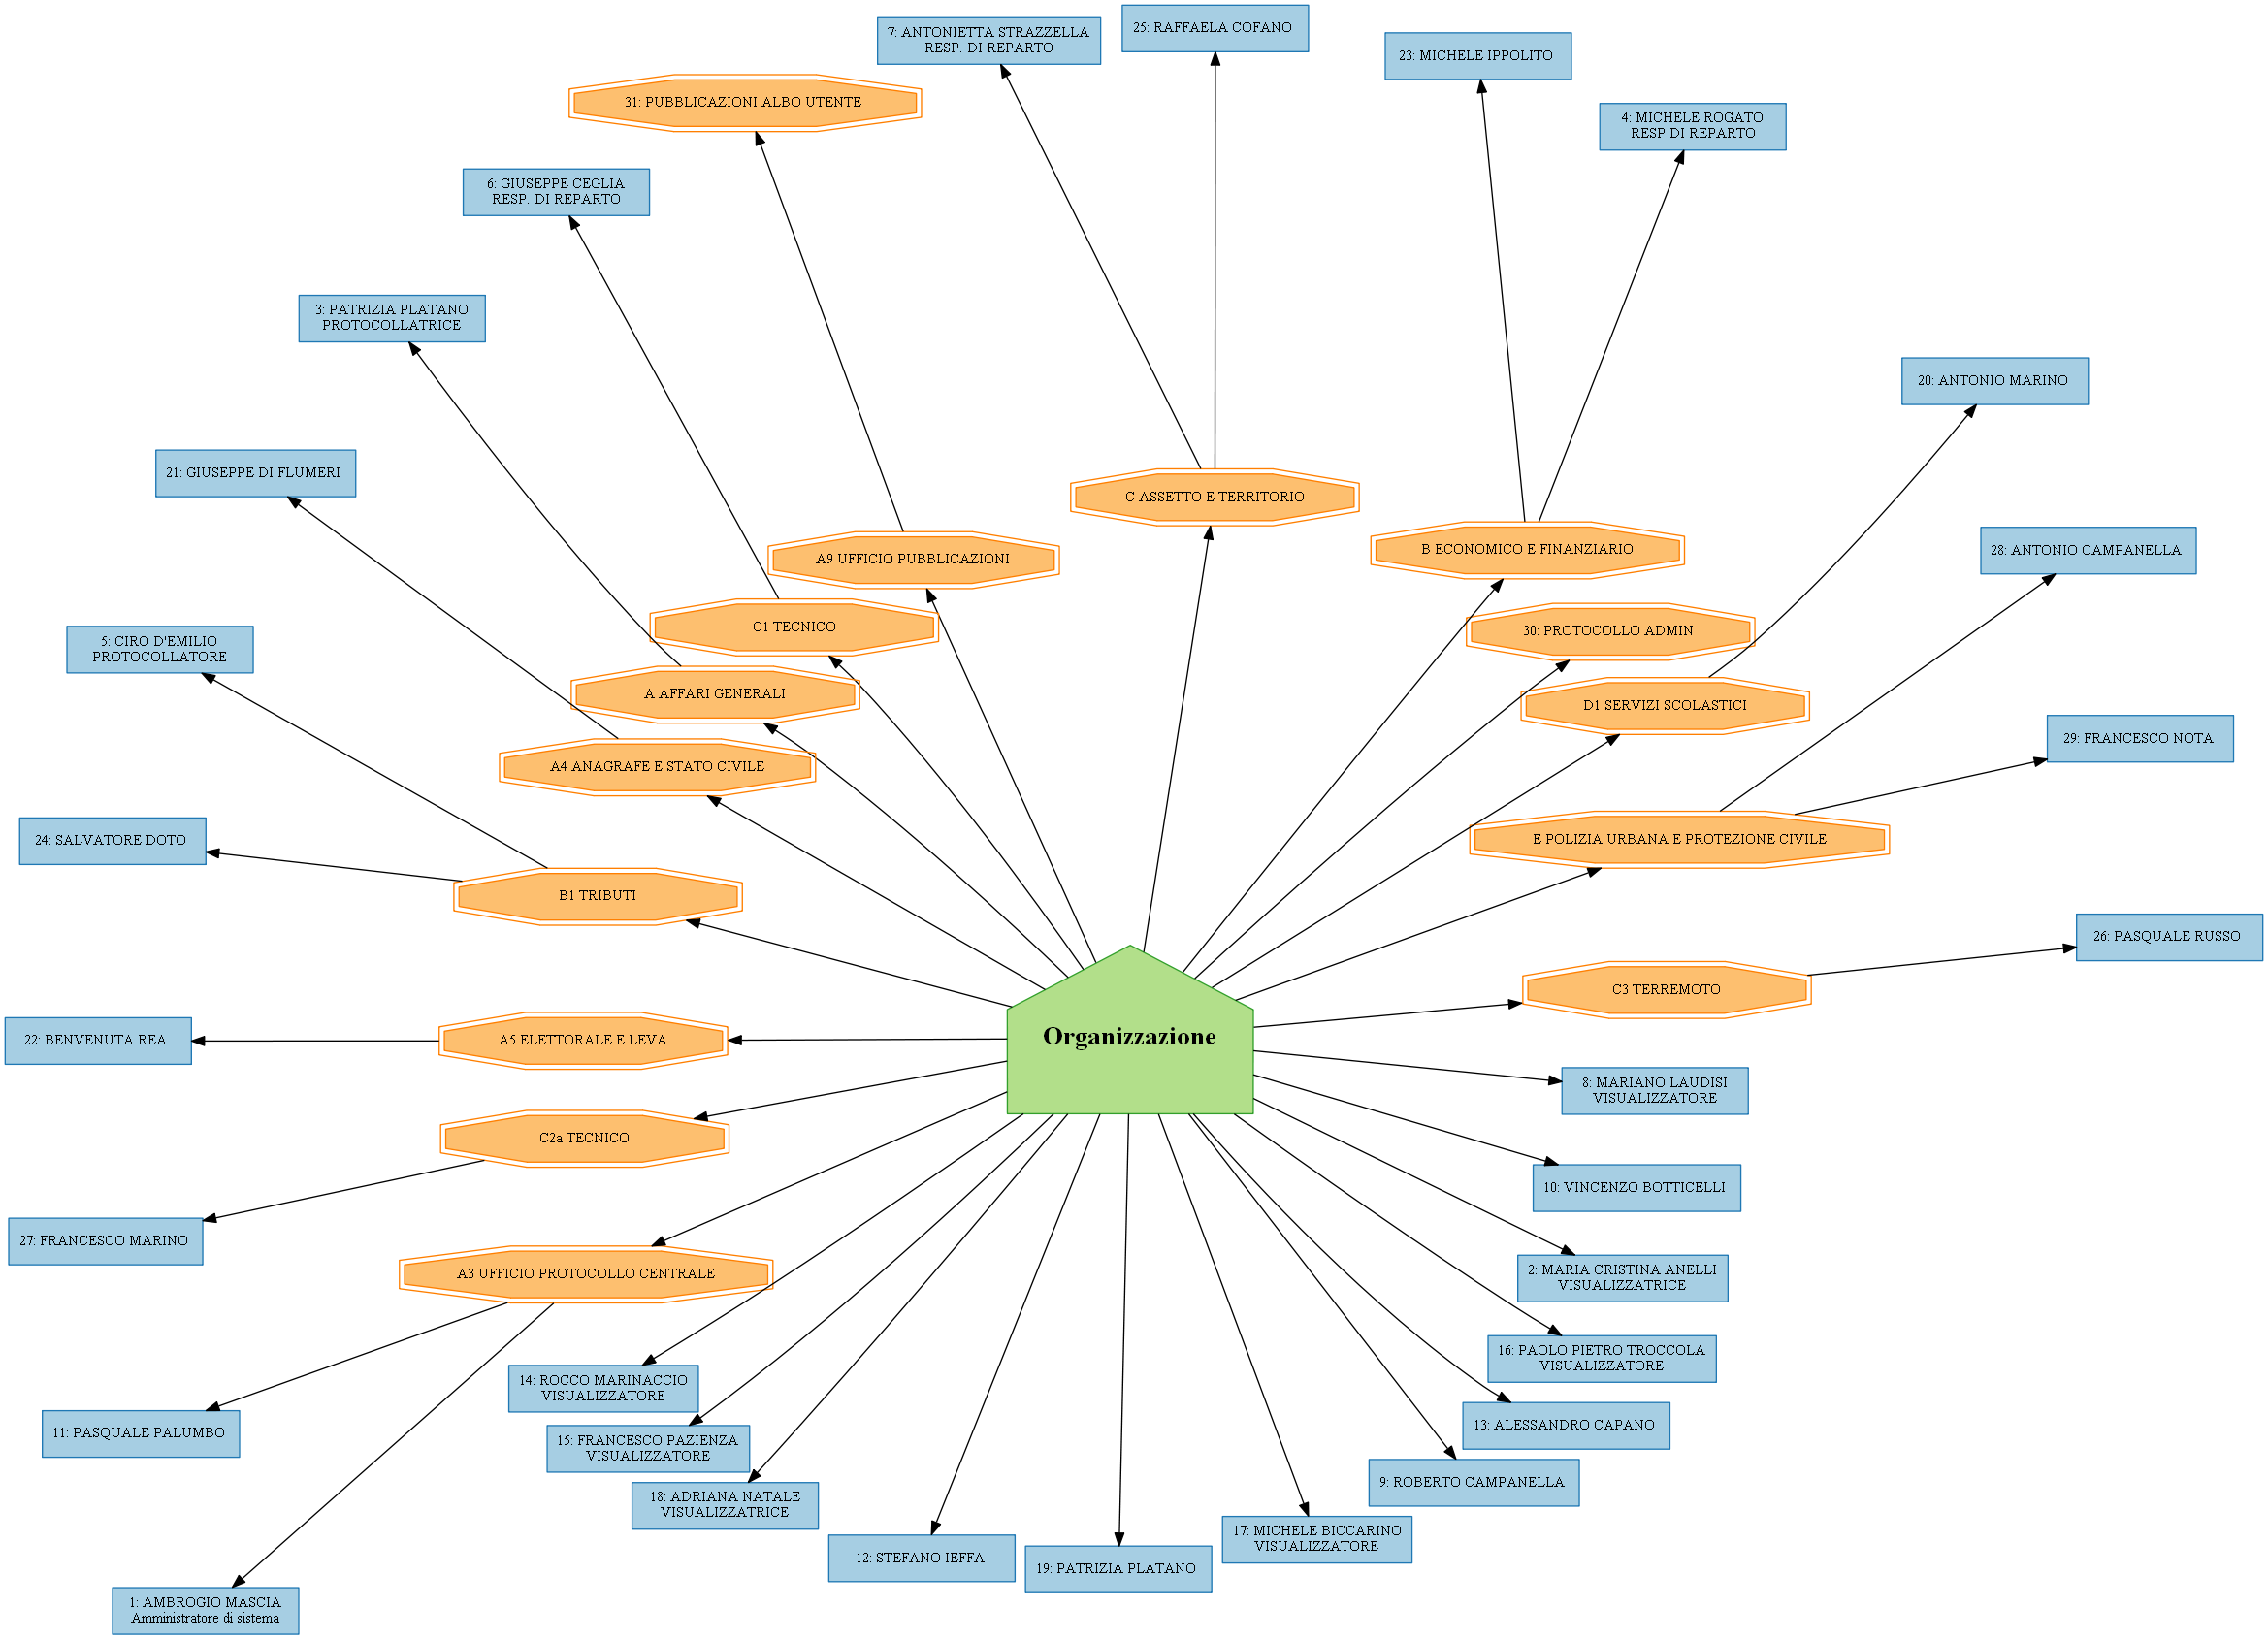
\includegraphics[width=14cm, height=6cm]{images/twopi.png}
		\caption{Typischer twopi Graph}
		\label{twopi}
	\end{center}
\end{figure}

\subsection{Vor- und Nachteile von Graphviz}
\subsubsection{Engines}
\subsubsubsection{Vorteile}
\noindent
Durch sechs verschiedene Engines kann man eine Vielzahl an verschiedenen Graphen erstellen. Wenn man genug über seinen Graphen in Erfahrung gebracht hat kann man die eine Engine die für seinen Graphen am besten passt auswählen und somit ein ideales Ergebnis erzielen.

\subsubsubsection{Nachteile}
\noindent
\begin{itemize}
	\item Jedoch der große Nachteil von Engines ist das man gebunden ist an sie. Man kann Beispielsweise nicht festlegen wo ein bestimmtes Element positioniert werden soll.
	\item  Außerdem kann man nicht bestimmen welche Größe die einzelnen Elemente haben sollen, da sie sich, je nach ihrem Inhalt, dynamisch anpassen.
\end{itemize}

\subsubsection{Formen}
\subsubsubsection{Vorteile}
\noindent
Es existiert eine Vielzahl an Formen und Linien, wodurch einem Freiheit bei der Modellierung ermöglicht wird.

\subsubsubsection{Nachteile}
\noindent
Ein Nachteil ist das man in seiner Freiheit eingeschränkt ist.
\begin{itemize}
	\item Will man eine neue Form festlegen, geht das schlicht und einfach nicht.
	\item Will man Text in einem Element unterstrichen haben, geht auch dies nicht.
	\item Beim modellieren hat man die freie Auswahl über schon vorhandenen Formen, jedoch um eigene Formen dann selbst zu erstellen bedarf es viel Arbeit und selbst dann ist das Ergebnis nicht zufrieden stellend und nicht immer das selbe.
	\item Ein anderer Nachteil ist, dass man wenn man ein Element verändert z.B.: einen anderen Rahmen gibt, dann wird das als neuer Standard angenommen und man muss, wenn man einen Sonderfall behandelt der selten vorkommt, jedes mal wieder den alten Standard festlegen.
\end{itemize}


\subsubsection{Dateiformate}
\subsubsubsection{Vorteile}
\noindent
Manche Dateiformate, wie z.B.: JSON, bieten einem die Möglichkeit nur auf die Informationen eines Graphen zuzugreifen die man auch wirklich benötigt. Das ist praktisch für Fälle wobei Graphviz nicht zur Darstellung verwendet wird sondern nur um das Layout festzulegen. 

\subsection{Vergleich von dot und neato}
\fib{}
\noindent
Die dot Engine erstellt hierarchische Graphen und die neato Engine gerichtete Graphen.
In der Regel wird dot häufiger genutzt, jedoch ist neato für Entity-Relationship Diagramme weit aus besser geeignet.
\footcite{graphviz_neato}

\subsubsection{Weingut}

\begin{figure}[H]
	\begin{center}
		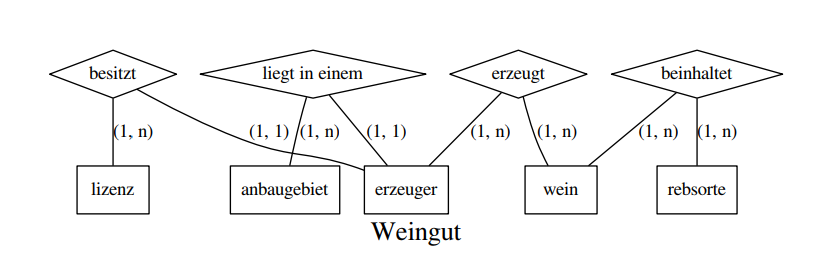
\includegraphics[width=16cm, height=8cm]{images/weingut_dot.png}
		\caption{Weingut mit der dot Engine}
		\label{wein_dot}
	\end{center}
\end{figure}

\noindent
Wie man an der oberen Abbildung \ref{wein_dot} sehen kann wäre dot für kleinere Graphen wie hier für dem Weingut durchaus denkbar. Solange Graphen nicht zu groß und nicht mehr als zwei Ebenen besitzen ist dot eine akzeptable Möglichkeit den Graph darzustellen.


\begin{figure}[H]
	\begin{center}
		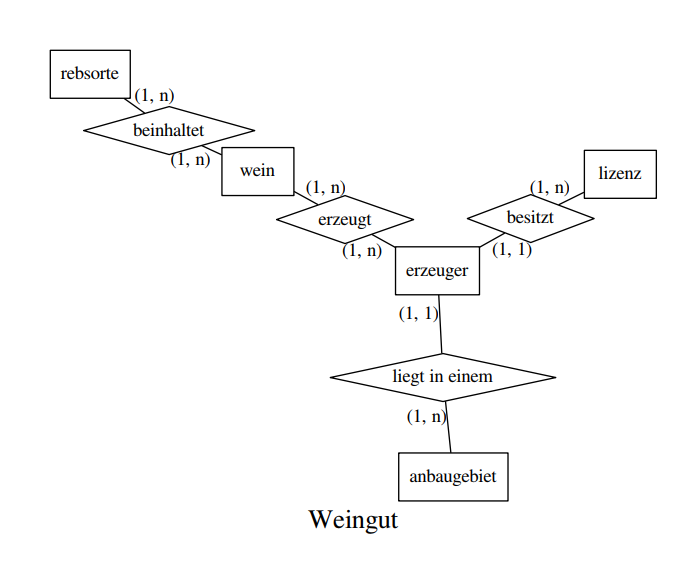
\includegraphics[width=16cm, height=8cm]{images/weingut_neato.png}
		\caption{Weingut mit der neato Engine}
		\label{wein_neato}
	\end{center}
\end{figure}

\noindent
Genau wie dot hat auch neato keinerlei Probleme mit kleinen Graphen wie dem Weingut.

\subsubsection{Rettungsstelle}

\begin{figure}[H]
	\begin{center}
		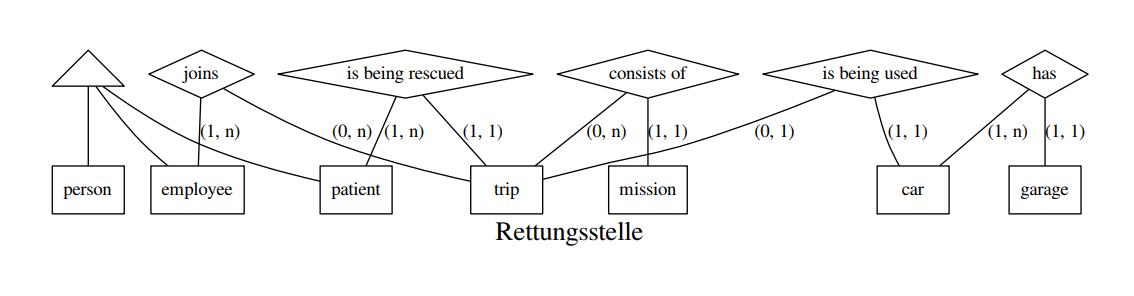
\includegraphics[width=16cm, height=8cm]{images/rettungsstelle_dot.png}
		\caption{Rettungsstelle mit der dot Engine}
		\label{rs_dot}
	\end{center}
\end{figure}
\fib{}
\noindent
Jedoch bei einem etwas größerem Graphen sieht man schon das dot zu breit wird und für Attribute keinen Spielraum mehr lassen würde.

\begin{figure}[H]
	\begin{center}
		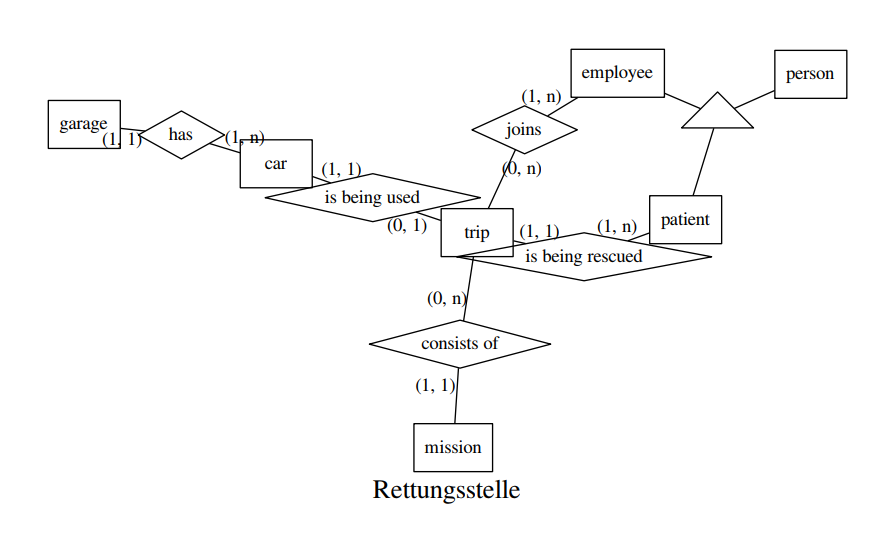
\includegraphics[width=16cm, height=8cm]{images/rettungsstelle_neato.png}
		\caption{Rettungsstelle mit der neato Engine}
		\label{rs_neato}
	\end{center}
\end{figure}

\noindent
Bei neato merkt man, wie hier bei der Rettungsstelle, dass noch Platz für Attribute wäre. Trotzdem merkt man das die Elemente immer näher aneinander rücken da der Graph für neato nicht die ideale größe besitzt.

\subsubsection{Wahl}
\fib{}
\noindent
Wenn man zwischen dot und neato wählen müsste sollte man vorher genaue Daten über den Graphen, den man generieren will, in Erfahrung bringen. In der Regel gilt beide eigenen sich für kleinere Graphen jedoch tut sich dot mit Attributen schwer und neato mit vielen Elementen. Bei vielen Elementen kann man aber auch sfdp benutzen da es neato ähnelt und auf größere Graphen ausgelegt ist.